\section{The Student Software Development Team}
Over a five year period, the Student Software Development Team (SSDT) has been employing students as software developers, to develop applications for an academic institution. The following framework is a generalization of the SSDT program. Following best practices in lean thinking \cite{lean}, the framework is constantly re-evaluated, redesigned, and optimized each year. Thus, the framework presented in this section represents its current state. It will certainly change as needs of the team and the institution evolve. The team also follows Agile principles \cite{agilemanifesto} . Figure~\ref{fig:framework} illustrates the framework, based heavily on Agile.

\begin{figure}[htbp]
 \centering
 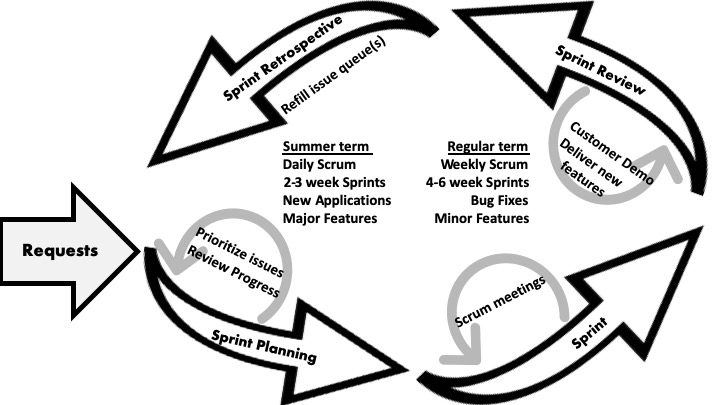
\includegraphics[width=\linewidth]{developmentcycle4.jpg}
 \caption{The SSDT's process for developing software}
 \label{fig:framework}
\end{figure}

The team also uses a modified version of Scrum \cite{thescrumguide}, which defines three key roles. The \textbf{product owner} is are the people who make a software request and are the customers who determine the vision the software. All decisions must be approved by the product owner before it is implemented. The \textbf{development team} consists of undergraduate students who are developing the software solution. Finally, the \textbf{Scrum Master} is charged with empowering the development team, communicating the needs of the product owner, and ensure constant forward progress. In the SSDT, the Scrum Masters are faculty or staff at the institution.

Scrum also describes four events: sprint planning, the sprint, sprint review, and sprint retrospective. These events are implemented differently in the framework depending on the term. In the summer, a more traditional Scrum model is followed with a product backlog and work in progress determined during sprint planning, daily Scrum meetings occurring during the sprint, and a sprint review and retrospective happening every two to three weeks. In the regular term (i.e., 16-week Fall and Spring terms), the Scrum timeframe is stretched out due to students working only 10 hours per week instead of 40 hours per week. Daily Scrums become weekly, and sprints take four to six weeks. Because the regular term is significantly less hours than the summer, only smaller features and bug fixes are expected during the regular term.

%new systems and major features are reserved for the upcoming summer term, while  

This next section describes our framework during the Summer Internship Phase, followed by the Maintenance and Customer Support Phase which occurs in the Fall and Spring terms. 

\subsection{The Summer Internship Phase}
During the summer, students are hired into the SSDT. Students apply in the previous Spring term, and are hired based on a few metrics: grades in core classes, such as CS1; their ability to work well with others (based on their interactions with other students in classes); and the value they will attain from participating in the program (i.e., the best computer science students are not always selected, as they may not benefit as much from the program). 

The Summer Internship Phase operates much like an industry internship, where students are employed for 40 hours per week for eight to ten weeks, resulting in up to 400 hours of experience. Six to ten students managed by Scrum Masters, (one faculty, one staff) work in pairs as they design interfaces and develop code following our Agile and Scrum framework. 

%%CUT? Their expectations mirror an internship in many ways, in that they are expected to show up at work on time, be productive throughout the day, and report back to supervisors of their progress. 

% CUT 4p Contrary to standard internships, the students do not spend a significant amount of time in ``training'' but instead are taught using a  ``just-in-time'' learning principle. The students are given only as much theory and knowledge about software engineering as is needed to begin the task at hand. 

%%For example, rising seniors will have completed CS2 and maybe a few upper level CS courses, while rising sophomores may have only had CS1. 

%%CUT?Very rarely will a student have been explicitly trained on software engineering principles, such as Agile methodologies, Model-View-Controller (MVC) or similar frameworks, or large-scale application development.

%%% CUT? For example, one of the first skills students must develop is the ability to work in a version control system, in our case, Git. Students are walked through Git basics, such as how to clone the repository, make commits, and issue pull requests, and then they are given their first issue from the issue queue. Their first issue is often selected very intentionally by the supervisors; for example, finding and fixing a typo in a README of one of the repositories. This gives them the confidence to make a change and issue a pull request to the repository owner, without the fear of breaking any system. 

%%% TODO: MOVE ME this is about the software and how they are obtained; the rest of this section is about the students process. %%%%%%%%%%% The projects are proposed by the campus community (a.k.a. the customer) and are then selected by the faculty member supervising the team. These projects are often tools requested by the customer to help them complete their daily work, and thus, the software becomes an crucial part of the customer’s job. 

A key skill gained by our students very early in the summer internship is the ability to translate customer's needs into usable software (i.e., requirements gathering and design). Students begin by designing the application on paper, known as paper prototyping \cite{2003paperPrototype}. This design process consists of many iterations of interfaces on paper, critiqued and modified until there is a group consensus. Then, the product owner is invited to demo the paper prototypes. This avoids the students spending significant hours writing code that doesn't match the team's understanding of the application or the product owner's needs.

%%% CUT At the beginning of this process, when students are still very new to the idea, the Scrum master will act as the "driver," meaning they "click-through" the interface drawn on paper by the students, while those who designed the prototype will move pieces of paper, representing new parts of the interface, to act out its functionality. The first draft typically acts as an eye-opener for the students; the driver will find many flaws and functionalities that their designs are missing. These design mistakes are noted, and the students return to the drawing board to build another version on paper. After multiple iterations, review sessions, and the group approves of the interfaces, the product owner is invited to demo the entire paper prototyped application. Once the product owner's feedback is recorded and taken into account when making the next version. When the interface is finally approved, the paper prototypes are video recorded for later reference (i.e., during coding). 

After paper prototyping, the students construct the database supporting their prototypes. As a group, they participate in a model building session in which they propose the underlying data structures of the application and the relationships between parts of the model. This process provides students with a better understanding of the models when they begin implementing their prototypes, reducing confusion about how data is saved and retrieved.  %%Again, many of the students have never taken a database design course, requiring more just-in-time training.

%%%CUT Multiple design iterations along with guidance from the supervisors lead to the students designing a working database which will support their paper prototypes. 

Having a design in place and an understanding of the data model, the students are ready to build the application. Students are given a VM and a bare-bones template for the application, with only as much code written for them as is necessary to begin writing code. They then embark on the development process, again following the framework from Figure \ref{fig:framework}. Students always work in pairs, following pair programming pedagogy \cite{2002PairProgramming}, which has proven particularly valuable for programmers learning a new language. 

%%% CUT (again, a skill they may not have learned in their courses yet).  For example, a main page may be constructed, with minimal content in it, and a basic query to the database to fill it with some dynamic content. From there, the student pairs must replicate the structure of the view and controller into their own interface.

During sprints, students meet each morning for a daily Scrum meeting. Students are encouraged to ask questions during the meeting. In fact, most of the training happens as a result of questions, since the team does not spend significant time doing formal training. As the summer progresses, the students learn to ask each other for help, promoting sharing of knowledge among team members. To maintain organization and visibility about what features each team is working on, we leverage Kanban boards \cite{anderson2010kanban}. Applying the Kanban model in tandem with the Scrum framework, also known as Scrumban  \cite{ladas2009scrumban}, aids in managing the overall flow of projects. 

% CUT 4p As the students' capabilities improve, questions become more technical in nature. During the daily Scrum, the students are encouraged to present their incomplete interfaces early in order to get feedback about components that may impact future code. Last, code is reviewed to demonstrate good and bad coding practices with the intention to catch flaws, misconceptions, and problems early on to keep software agile and easily adaptable.


% CUT 4p Figure \ref{kanban} shows the most recent iteration of our Kanban board (which has changed many times as the team finds ways to improve its usefulness).
%seems like this board needs to be explained more for it to be here -kat 10/28/19
% \begin{figure}[h]
%  \centering
%  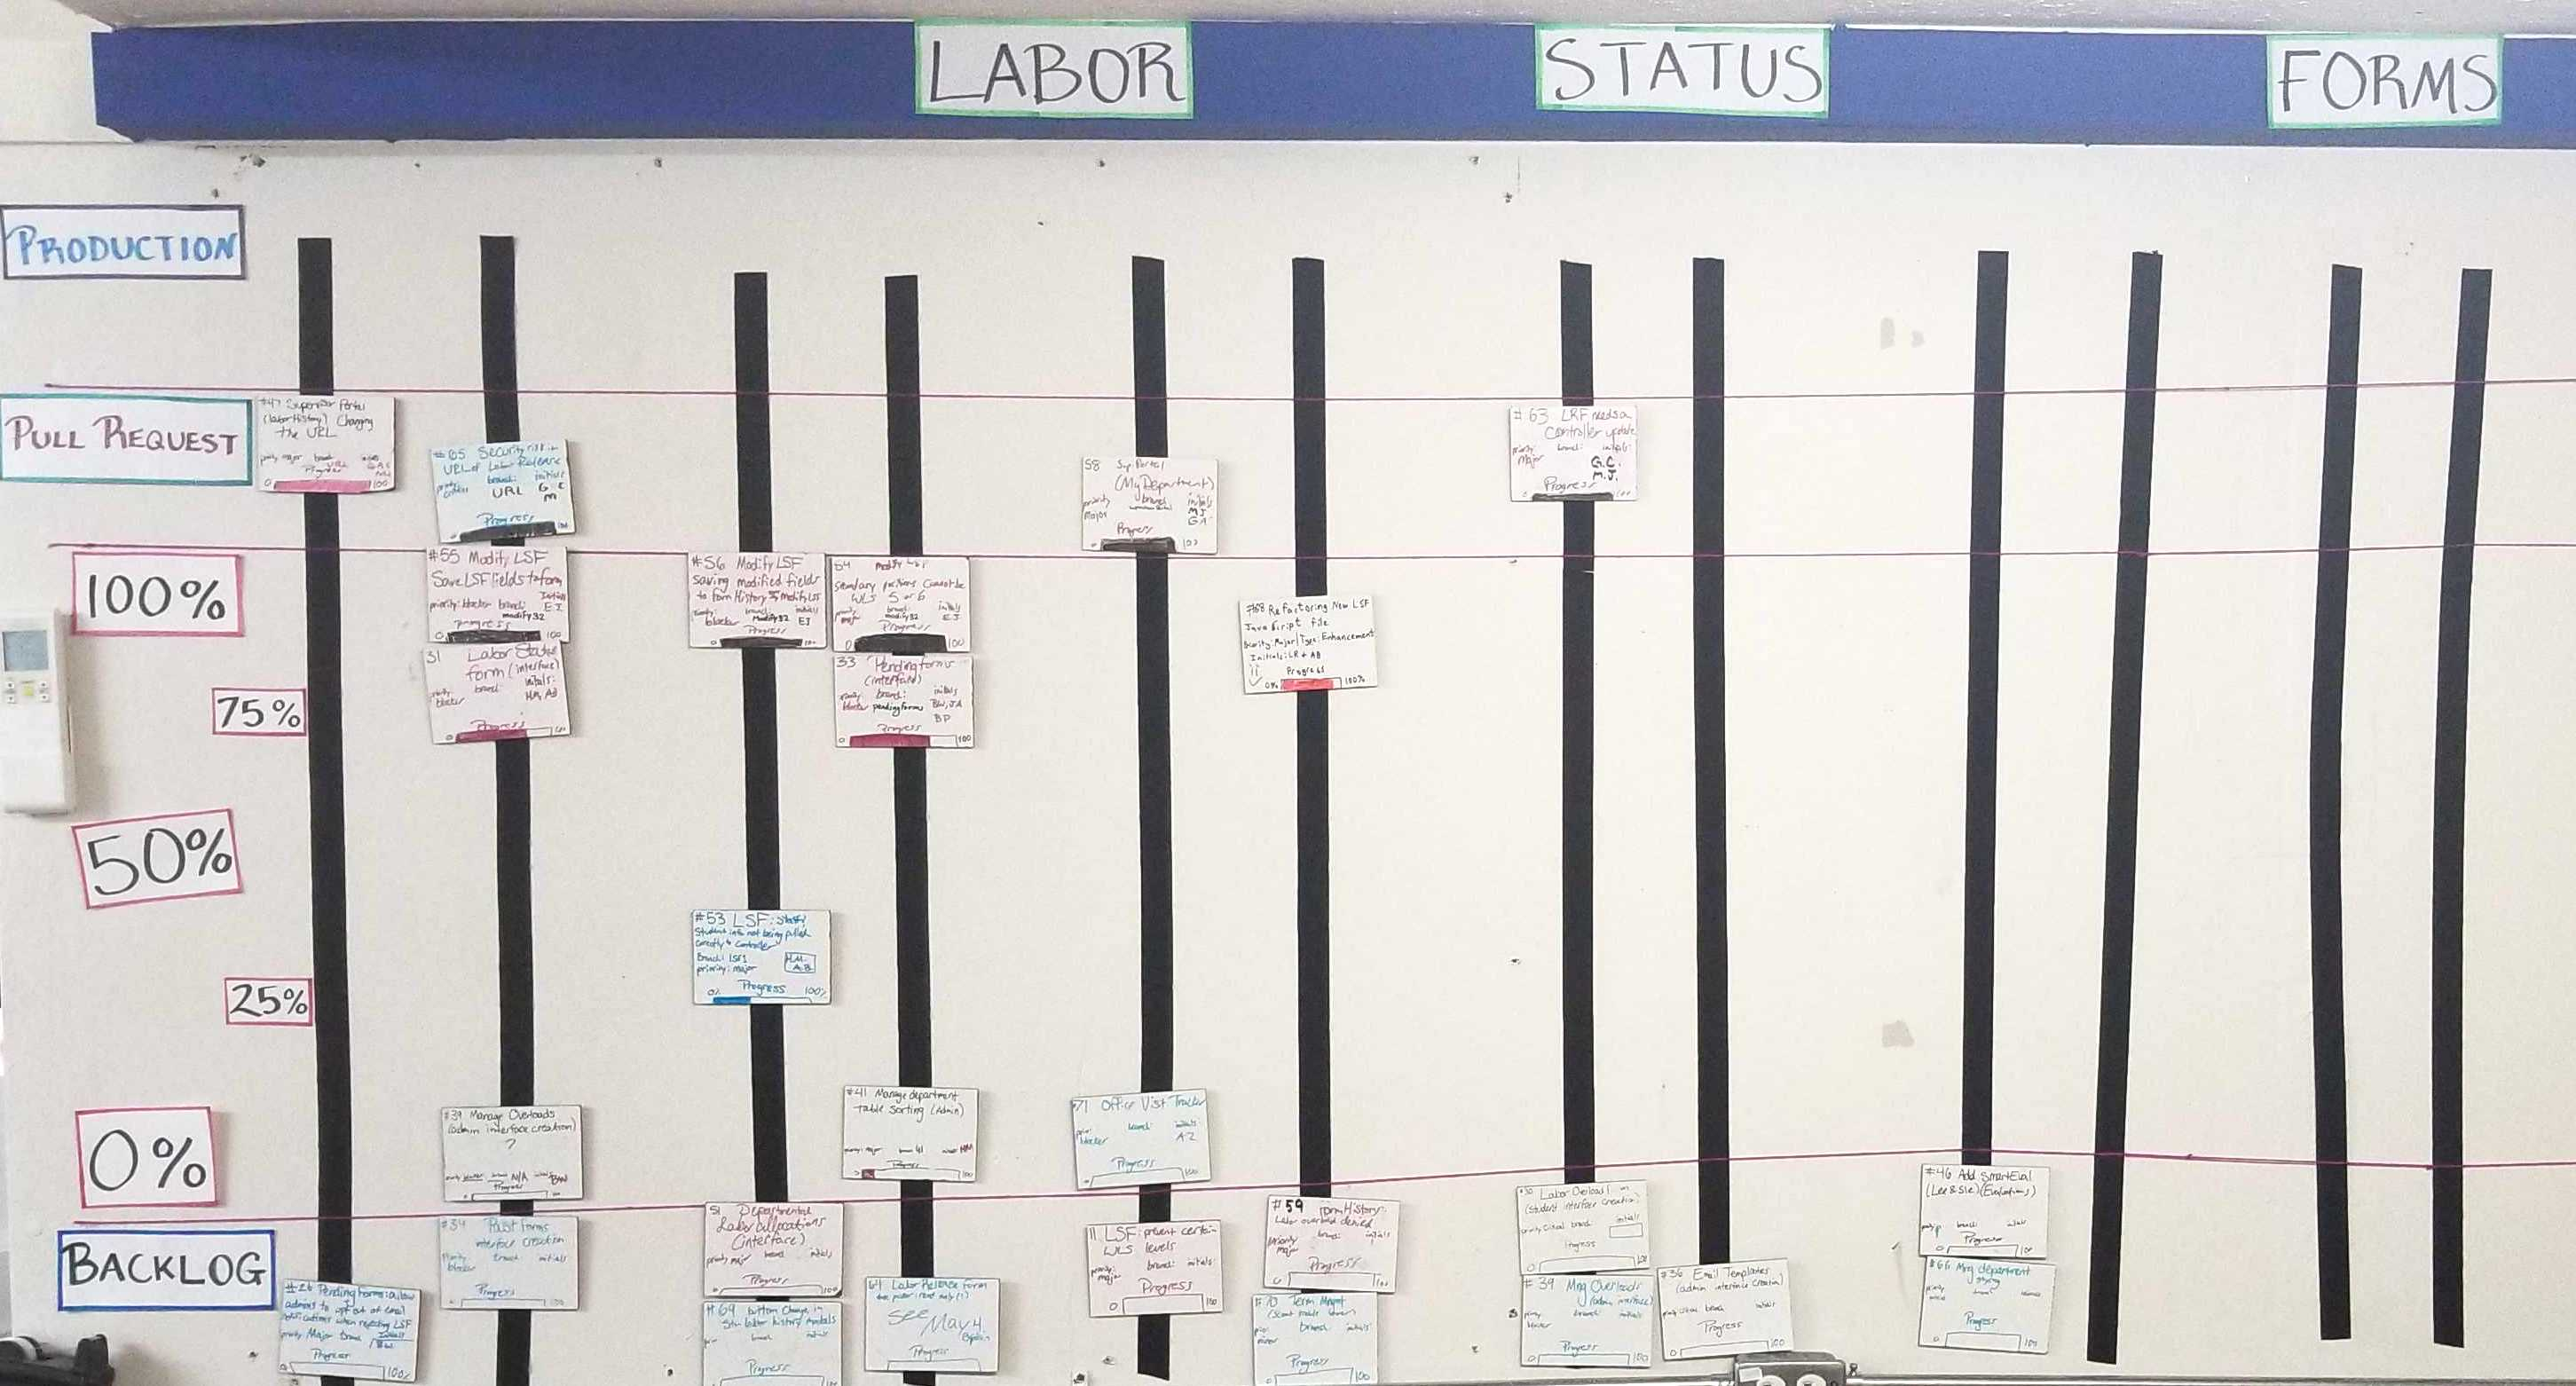
\includegraphics[width=\linewidth]{kanban.jpg}
%  \caption{Kanban board for organizing team progress}
%  \label{kanban}
%  \Description{Kanban board for organizing team progress}
% \end{figure}

%%%CUT? Another important tactic in promoting the sharing of knowledge involves rotating teams. The team lead and supervising faculty member conduct a meeting a few weeks into the summer term to evaluate each pair's performance. They evaluate each developer's strengths and weaknesses, then redistribute the teams. Typically one developer stays on the interface they were already working on developing, and gain a new partner who is new to the interface. Shuffling the pairs helps students be flexible, learn to collaborate with others, and most importantly, reveals the importance of well-documented code and following coding standards adopted by the team. It also encourages the students to be able to explain their progress, clearly articulate their goals, and know exactly what their code does as they explain it to their new partner. 

Pairs begin conducting usability tests \cite{usabilitytesting} to ensure that their interface is user-friendly. The pair will conduct a usability test first with a team who has not used their interface, then with the Scrum Master, and lastly with the product owner to get their final approval of the implementation. Then, the students' code gets tested for security, coding standards, and bugs before being integrated into the production environment. 

%%% CUT 4p The hosting team provides a set of tasks or scenarios to complete, then observe the user. Usability tests showcase previously unseen faults or unconsidered scenarios in their interfaces thus far. For example, during development, teams will commonly only test the expected use case. The usability test might reveal that there is another set of operations that the user can do which causes a crash. After fixing these new bugs or improvements, they will conduct another usability test, typically with . %%%It is expected that there will be less (but rarely none) new bugs or usability problems to fix. 

Ideally, a full product is delivered to the product owner by the end of summer. Good communication with the product owner and clear expectation setting alleviate issues with surprises about delays in deployment, which are inevitable. Features that aren't completed become issues for the team to solve during the regular term. 

\subsection{The Maintenance \& Customer Support Phase}
In the fall term, the team shifts to weekly (instead of daily) scrum meetings and a 10-hour work week, as the students are attending classes in addition to working. As expected, productivity reduces dramatically compared to summer. The framework takes this into consideration. Now the team focuses more on maintaining existing software and responding to customer needs (e.g., bug fixes or small feature requests). Students gain the valuable experience of having to maintain their software after deployment, a skill rarely taught in software engineering courses or capstones after projects are ``completed.''

% Students are expected to schedule their hours so that no student is working alone for extended periods of time. Students who work alone for too much of their time develop bad coding habits, make poor design and usability choices as they implement if there is no one there to brainstorm solutions with them. The Scrum Master typically isn't available to assist the students as quickly as they did during the summer so students must rely on each other more-so than before. 

Work duties are mostly determined by the users (as they encounter bugs) and the product owner (as they start thinking of new features they want in their software). New issues are added to the issue queue for that application as they are reported. Urgent issues (e.g., causing crashes or rendering an interface unusable) are taken by the first available student. Non-critical issues are discussed in the weekly scrum meeting and added to a team's work in progress, or left in the issue queue for the next week. 

% Back to the kanban board...
%%%CUT 4p 
Similar to summer, the Kanban board is key in keeping the team organized and aware of each others' work. Students check the Kanban wall for new issues, claim them, and keep record of their progress. This helps the students avoid duplication of work and visualize progress. When an issue is resolved and tested, a pull request is issued and reviewed by the Scrum Masters. An accepted pull request must pass guidelines for security, accessibility, and coding best practices. The Scrum Masters are then responsible for integrating the feature into the production environment.  

As the Spring term ends, some students graduate and others leave the program, but a few students will continue into the second or third year. The next summer student cohort is selected based on available seats in the program, and the next set of major features or new systems are selected for that summer. The staggering of students enables knowledge transfer, as more senior students in the program will mentor new students, creating a knowledge pipeline from year to year. Note that the SSDT does not deliver software and then not support it; each new system becomes the responsibility of the next cohort to maintain, on top of the systems and features they create.

% CUT 4p \section{The Software}
% Quick paragraph... improve?
% CUT 4p This section begins by describing the process for selecting new requests for software, followed by a brief summary of the structure the current software that has been generated by the SSDT has been built upon. Lastly, two examples of applications built by the SSDT are presented.

% CUT 4p \subsection{Selecting Software Requests}
% CUT 4p The team receives software requests from departments and offices at the institution who are aware of the Student Software Development Team and think we can help them. In some cases, the department needs to replace old or inadequate software they already own. In other cases, they are still relying on inefficient paper processes that could easily be replaced with a software solution. It is also not unlikely for team members to reach out to departments and inquire about their needs. When a software request is received, the team reviews the request and determines which projects are feasible and which lie outside of the mission of the team. Selected projects go into a backlog to be considered in the upcoming summer. A number of factors determine which systems we will implement, including the request's urgency, value to the institution, and the expected effort required to complete the project. All of these factors are weighed in order to select the request that best fits our capabilities and current capacity.

% % CUT?
% \subsection{Software Engineering Principles}
% After a software request is selected, the summer term starts with the team following the principles and values described in the Agile Manifesto to begin building the software solution. The Manifesto does not provide concrete or descriptive instructions on how to develop software, but instead provides fundamental information to be considered throughout the entirety of the software development from project initiation to project close. Agile software development prioritizes interactions within the software team as well as with the customer, and encourages software processes that are receptive to change while still delivering quality software \cite{agilemanifesto}. % How are we using it?

% % CUT The hybrid of Scrum used by the team also intertwines the Kanban model into its practices.
% Scrum methodology is a subgroup of the Agile project management framework that articulates more details and specifications on how to employ the principles in the Manifesto within the team's software development practices with ``the goal of delivering new software capability every 2-4 weeks'' \cite{thescrumguide}. [BRIACHECKTHIS] Scrum is the most popular agile methodology; ``According to the 12th annual State of Agile report, 70 percent of software teams use Scrum or a Scrum hybrid'' \cite{}. 



% Cut? The four Scrum events complemented with Kanban references these events as ``flow-based events'' to acknowledge the importance of managing the teams workflow during these events. The Summer term, when students work for 40 hours a week, is when the team can execute these events to the full extent as the team is able to convene in a way that is comparable to that of a software team that works full-time year round. The Sprint Planning begins when the team decides which customer request will be the central focus for that year. This event is used to outline the work that will be performed during the Sprint. The Development Team uses this time to forecast the range of capabilities that will be developed during the Sprint and to also set the Sprint Goal. The Sprint Goal for the SSDT is to have a beta product available by the end of the Sprint. When a software is released in beta, the majority of the software requirements have been met, however,there may be small issues that have yet to be addressed. By releasing beta versions of products, the SSDT and the Product Owner are able to observe most of the functionality of the software that has already and also test for inconsistencies. Close communication with the customers is crucial to the development of the software; staff's needs may change, college policies may update, and staff may move on to jobs elsewhere. As needs change, SSDT can adapt to and account for them.

% Repeat of above words
% \paragraph{Sprint Planning \& Paper Prototyping}
% Sprint Planning begins with analyzing the current processes that the Product Owner is utilizing*. Asking questions such as, What does the current software that is used to solve their problem look like? How does it work? Are they using any software? Where is the data that needs to be tracked currently being stored? What forms have to be filled out and which people have the authority to approve this process before it is considered to be done and put into action. For instance, if the Product Owner was requesting a software that allows students to add and remove courses to their schedules. The SSDT would need to know how students are currently able to do this task and then make sure to add it to the requirements of the software that is being built. During the SSDT's most recent Sprint, the request that was chosen involved doing an entire refactoring of a live* software.

% In order to get a better idea of the functionality of the new software should be implemented, the Development Team begins by going through multiple iterations of paper prototypes. Paper prototyping is a prototyping method in which paper is used to simulate a computer or web application. A paper prototype should hold all of the functionality that the finished user interface of the application will have; from navigation bars, drop down menus, and headers to button clicks and items that will hover on the interface. A person should be able to ``click-through'' the website via the paper prototype. To start this process, screenshots of the old software's interfaces were taken and printed out. Next these interfaces are critiqued* and analyzed to decide which parts are to be kept for the refactoring, which parts will need to be reworked, and which parts will need to be discarded altogether. The purpose of this part of the paper prototyping process is to become familiar with the current software so that the team can adequately build a better software. The team looks for things* such as bugs, broken links, slow page loading, poor user design, etc. and makes a note of these issue to ensure that they are addressed in the new software. After the individual interfaces of the previous software have been discussed and analyzed, the team divides the different interfaces into two categories: Main and Administrative. Main interfaces are the web pages that all users of the application will be able to see whilst Administrative web pages will only be accessed by system administrators, such as BC staff and SSDT's supervisor.

% Next the team breaks down the interfaces into issues in which the team will tackle* in pairs. The pair of developers then begins to design the interface that they had chosen from the interfaces that needed to be refactored. Each time a pair from the team believes that they have successfully created a valid* paper prototype, it is then tested for usability. Paper prototyping testing occurs* in the same way that a fully functional software would be tested, the person testing the paper interface will treat it as such. The tester will ``click'' on different components of the interface and the designers will physically move parts and replace parts of the paper interface in order to replicate how the real software would respond. The pair who designed the interface will take notes as the tester navigates their paper web page and when the test is complete, they use these notes to redesign and the process is repeated. Paper prototyping is done because ``bug'' and inefficiencies are easier to fix when no coding has been done yet and one can go through many iterations without having to actually having to troubleshoot actual code. The SSDT repeats this process of designing, testing, and re-designing until the entire team is satisfied with the final iteration. After all interfaces have been drafted and prototyped, the process of building the application begins and the team commences the Sprint.

\section{Software Built by the Student Software Development Team}
% \subsection{Software Built by the Student Software Development Team}
The vast majority of the applications created by the SSDT are browser-based web applications. The SSDT follows an MVC architectural model to structure all of the applications. The team uses Flask, a web framework that uses Python as a back-end language (i.e., the controller), designed to make the start-up of a web application quick and easy. Coupled with two Python libraries, Jinja for template rendering (i.e., the view) and Peewee for database abstraction and integration (i.e, the model), the team has all of the tools needed to begin building web applications. Since most of our applications are intended to be tools for doing work (as opposed to web sites for selling products or advertising services), we leverage Bootstrap for web page styling and simplifying the implementation of the front-end of the application, particularly related to mobile-readiness and responsiveness. The database is hosted in a MySQL server. 

In the five years since the creation of the SSDT, we have developed twelve software systems: three are retired, and one is not maintained by the SSDT any longer. The remaining eight applications are regularly maintained by the SSDT. For brevity's sake, we will describe only one of these applications that are of relevance to many academic institutions.

% CUT (may belong in AY section) Communications with the product owners occur at a minimum twice a year, where new features are proposed. Otherwise, customers report bugs and issues via email to the SSDT, which enter the issue queue and get resolved by the team as quickly as possible.

%Systems: Advancement, BCAC, BCSR, CAS, LSF, Skyz, Ulmann, Urcpp, EDDY (ret.), BART (ret.), GoIntern (ret.), Sustainability (no maintenance)

\subsubsection{The Chemical Inventory System} %skyz
One responsibility of the Environmental Health and Safety department is to track and control the movement of hazardous chemicals on campus. Chemicals must be stored in a special bunker, and certain regulations exist for certain chemicals. The institution was managing the chemical inventory through dated software which was slated for retirement. The department needed a new solution, but was not given an adequate budget to purchase existing solutions that served their exact needs. The SSDT was approached to implement a solution which solved the needs specifically for the department. 

The SSDT created a web application allowing the department to track all chemicals on campus. The application had the added benefit of providing access to interested individuals (e.g., chemistry faculty) to view the current stock of each chemical, and see details about the chemical (e.g., expiration date). The system was extended to include the ability to generate reports (i.e., in case of emergencies, such as a fire), as well as document the disposal of chemicals. In all, the software made the campus safe, improved visibility about the inventory, and resolved years of inconsistent data the old tool.

% CUT 4P \subsubsection{Course Administration and Scheduling (CAS)}
% Originally, the Registrar's Office would send an email out to all of the department chairs at the institution requesting the schedule for upcoming terms. Department chairs would then respond to the email with their drafted schedules. This data would get aggregated into a single spreadsheet by the Registrar, then emailed back out to the department chairs for review. This process would repeat for multiple weeks as department chairs resolved conflicts in scheduling (e.g., ensuring required courses from other departments not overlapping), each week requiring the Registrar to update the spreadsheet and resend it via email. To further complicate the process, additional approvals were required by other chairs and deans, as well as some courses not being as straightforward as others (e.g., special topics courses, cross-listed courses, team-teaching situations, prerequisites, co-requisites, to name a few). This process was error prone and inefficient for all parties involved. The SSDT was approached to develop a software solution that would improve the situation for everyone. 

% The SSDT developed the Course Administration and Scheduling (CAS) system, a web application that allowed department chairs to enter in all of the course information for their department. Each department chair had access to edit their own department, and could view the schedule of all departments as the schedule was being constructed. The application provided data validation tools to ensure only valid inputs were allowed (e.g., course numbers and titles matched the institution's course catalog), as well as the ability to handle all of the non-standard courses, as mentioned above. The Registrar was given the ability to lock the schedule at a specific dates. The full list of courses was then exported from our application and imported into the official schedule for that term. 

% The application was well-received, particularly by the Registrar's Office, who was no longer spending significant hours managing spreadsheets over email. The application has also survived multiple staffing changes, including a new Registrar and two new Assistant Registrars (who interacted with the software the most). In each case, the new staff members were able to learn the software quickly and integrated it into their workflow. The Registrar's Office has also requested new features and changes to existing features to be integrated into the system since its creation. For example, a matching algorithm was added to facilitate a more unbiased approach to assigning rooms to classes without creating conflicts, particularly important for popular rooms where multiple faculty would lobby to be given that space.  

% The CAS application started as a simple scheduling tool, and has evolved over the last four years into a much larger application for managing multiple aspects of course scheduling, empowering faculty to have more voice in their room placement, and improving visibility of the larger schedule to the entire faculty and staff.
%%%%%%%%%%%%%%%%%%%%%%%%%%%%%%

% CUT During the Sprint, the team convenes everyday in the morning in order to touch base with each of the pairs within the team and get an idea of their progress. During the Scrum meeting, the smaller teams tell what the have accomplished since the last meeting, what they will begin to work on next and what they will be completing before the next Scrum meeting, and where they are stuck or if any obstacles got in the way of completing their previous work. Scrum meeting (also called the Daily Stand-Up) is for quick communication purposes and should take no longer than 15 minutes. Sometimes small demos are done during the Scrum meeting in order to get the entire teams' input on certain features before proceeding. The programmers are expected to do a ``DDS'' in a team collaboration application called Slack, DDS stands for Did, Doing, and Stuck. During the Academic Year, these updates serve to compensate the lack of daily Scrum meetings; all students are not available at the same time while classes are in session. Team leaders examine the DDS reports to ensure progress is steady as well as evaluate who needs guidance. These updates also aid in communication between team members if they happen to not see each other. Instead of having a daily Scrum, we instead have a weekly Labor Meeting in which we present and evaluate the team's progress and state in production.

% \paragraph{SPRINT REVIEW}
% The Sprint Review's purpose is to inspect the amount of work that was completed during the Sprint and measure the amount of work needs to be completed for the next Sprint. The SSDT uses a version control application called GitHub that allows them to edit parts of the software using a copy of the application in their own environment without interfering with the main program. When the Sprint is completed, the parts of the application that were successfully finalized during the Sprint are merged into the main program. This will allow the team to then create another copy of the main program that now has the new changes and fixes to include in the next Sprint. After the Sprint is completed, the team does an overall demonstration to present the work that they have completed during the Sprint. After the team demonstration, the Product Owner is brought in so that the team can present the work that has been completed so far. It is important that the Product Owner also participates in the Review; their job is to make sure the work so far meets their criteria and requirements. They also have the authority to reject part of the application, suggest modifications to what has been built, or request a feature be added to the application. The feedback from the Product Owner during this stage is essential as it defines new criteria for the next wave of implementation.

% The Review is also used to help set goals for the next iteration. The team holds another meeting to discuss what issues and features were supposed to be completed by the end of the Sprint, but did not. Of those issues, how close are they to being completed and what is a realistic goal that be set for completion in the next Sprint. The SSDT will also review the work that was added during the Sprint or the work was removed. This will give the team insights about what goals may have been too ambitious for the Sprint deadline and what goals could have had more tasks added to them. The Review helps the SSDT to transparently assess the capabilities of the team.

% \paragraph{SPRINT RETROSPECTIVE}
% This is the final meeting after the Sprint in which the team discusses the overall process and performance of the Sprint. The Sprint Retrospective provides an opportunity for the SSDT and the Scrum Master to strategize ways to improve their methods and approaches for the next Sprint. The objective of this part of the Scrum process is not to focus so much on the work itself but to evaluate the processes of the team. During the meeting, the team finds what activities worked well and should continue to be used in the future, what went wrong during the Sprint, and what could be improved for the next iteration. This meeting is not, however, designed to assess the performance of an individual or to penalize anyone for any shortcomings. The intention of the Retrospective is to gather information about ways to improve the next Sprint. During this discussion, the team openly explores the difficulties and challenges faced during implementation. The team's strengths and triumphs are examined alongside the setbacks to better prepare for these challenges in the future.

% \subsubsection{The Academic Term} 
% The Fall and Spring terms are both comprised 16 weeks* where most students work at least 10 hours a week. Upperclassmen students can work up to 15 hours a week, if permissible. In addition to class scheduling occupying the students' weekly routines, the weekly labor restrictions follow the guidelines established by the labor program at the institution.


% "MOVE ME" ``The SDDT at our institution was established over four years ago with the Student Software Development Initiative by a Computer Science faculty member.''

% "DONT THINK WE NEED THIS" ``Students learn real-world work skills such as time management, and responsibility. Some students move up into positions of leadership and build those skills. Between classes, extracurriculars, and secondary labor positions, SSDT's staff dedicate time to their labor hours.''
